\documentclass[11pt]{article}
% Shared preamble of the RMC kernel write-ups (% Shared preamble of the RMC kernel write-ups (% Shared preamble of the RMC kernel write-ups (\input{preamble} after \documentclass).
\usepackage[margin=1in]{geometry}
\usepackage{amsmath,amssymb,bm}
\usepackage{graphicx}
\usepackage{booktabs}
\usepackage{hyperref}

\newcommand{\dd}{\,\mathrm{d}}
\newcommand{\Ein}{E}
\newcommand{\Eout}{E'}
\newcommand{\Ecm}{E_{c}}
\newcommand{\mucm}{\mu_{c}}
\newcommand{\mulab}{\mu_0}

% Common closing section: how the verification figures are produced
\newcommand{\verificationmethod}{%
Each figure is produced by \texttt{verification/verify\_laws.py}. For an incident
energy $\Ein$ along $+z$, $10^6$ collisions are sampled with MC/DC's own reaction
sampler (\texttt{sample\_elastic\_scattering}, \texttt{sample\_inelastic\_scattering}
or \texttt{sample\_fission}), and every emitted neutron is histogrammed in
$48 \times 24$ bins of $(\Eout, \mulab)$, with $\mulab$ the lab cosine to $+z$. The
inverted kernel used by RMC is integrated over the same bins (Gauss--Legendre panels;
two-body lines are split where $\mulab^*(\Eout)$ crosses a cosine edge), multiplied by
the number of collisions, and compared with a $\chi^2$ test over bins with at least 5
expected counts (the rest pooled into one bin). The tables list $\chi^2/\mathrm{dof}$,
its $p$-value, the emitted neutrons per collision (sampled vs.\ the integral of the
inverted kernel), and the largest relative change of a bin integral when the
quadrature panels are doubled. Left panels: outgoing-energy marginal; middle:
lab-cosine marginal; right: per-bin $z = (\text{sampled} - \text{inverted}) /
\sqrt{\text{inverted}}$.}
 after \documentclass).
\usepackage[margin=1in]{geometry}
\usepackage{amsmath,amssymb,bm}
\usepackage{graphicx}
\usepackage{booktabs}
\usepackage{hyperref}

\newcommand{\dd}{\,\mathrm{d}}
\newcommand{\Ein}{E}
\newcommand{\Eout}{E'}
\newcommand{\Ecm}{E_{c}}
\newcommand{\mucm}{\mu_{c}}
\newcommand{\mulab}{\mu_0}

% Common closing section: how the verification figures are produced
\newcommand{\verificationmethod}{%
Each figure is produced by \texttt{verification/verify\_laws.py}. For an incident
energy $\Ein$ along $+z$, $10^6$ collisions are sampled with MC/DC's own reaction
sampler (\texttt{sample\_elastic\_scattering}, \texttt{sample\_inelastic\_scattering}
or \texttt{sample\_fission}), and every emitted neutron is histogrammed in
$48 \times 24$ bins of $(\Eout, \mulab)$, with $\mulab$ the lab cosine to $+z$. The
inverted kernel used by RMC is integrated over the same bins (Gauss--Legendre panels;
two-body lines are split where $\mulab^*(\Eout)$ crosses a cosine edge), multiplied by
the number of collisions, and compared with a $\chi^2$ test over bins with at least 5
expected counts (the rest pooled into one bin). The tables list $\chi^2/\mathrm{dof}$,
its $p$-value, the emitted neutrons per collision (sampled vs.\ the integral of the
inverted kernel), and the largest relative change of a bin integral when the
quadrature panels are doubled. Left panels: outgoing-energy marginal; middle:
lab-cosine marginal; right: per-bin $z = (\text{sampled} - \text{inverted}) /
\sqrt{\text{inverted}}$.}
 after \documentclass).
\usepackage[margin=1in]{geometry}
\usepackage{amsmath,amssymb,bm}
\usepackage{graphicx}
\usepackage{booktabs}
\usepackage{hyperref}

\newcommand{\dd}{\,\mathrm{d}}
\newcommand{\Ein}{E}
\newcommand{\Eout}{E'}
\newcommand{\Ecm}{E_{c}}
\newcommand{\mucm}{\mu_{c}}
\newcommand{\mulab}{\mu_0}

% Common closing section: how the verification figures are produced
\newcommand{\verificationmethod}{%
Each figure is produced by \texttt{verification/verify\_laws.py}. For an incident
energy $\Ein$ along $+z$, $10^6$ collisions are sampled with MC/DC's own reaction
sampler (\texttt{sample\_elastic\_scattering}, \texttt{sample\_inelastic\_scattering}
or \texttt{sample\_fission}), and every emitted neutron is histogrammed in
$48 \times 24$ bins of $(\Eout, \mulab)$, with $\mulab$ the lab cosine to $+z$. The
inverted kernel used by RMC is integrated over the same bins (Gauss--Legendre panels;
two-body lines are split where $\mulab^*(\Eout)$ crosses a cosine edge), multiplied by
the number of collisions, and compared with a $\chi^2$ test over bins with at least 5
expected counts (the rest pooled into one bin). The tables list $\chi^2/\mathrm{dof}$,
its $p$-value, the emitted neutrons per collision (sampled vs.\ the integral of the
inverted kernel), and the largest relative change of a bin integral when the
quadrature panels are doubled. Left panels: outgoing-energy marginal; middle:
lab-cosine marginal; right: per-bin $z = (\text{sampled} - \text{inverted}) /
\sqrt{\text{inverted}}$.}


\title{Inverted kernel: free-gas elastic scattering (thermal target motion)}
\date{}

\begin{document}
\maketitle

\noindent Applies to elastic scattering at $\Ein \le 400\,kT$ ($T$: nuclide
temperature), where MC/DC samples the motion of the target nucleus. Code:
\texttt{free\_gas\_density}, \texttt{free\_gas\_support}, \texttt{sample\_free\_gas}
in \texttt{mcdc/rmc/reaction.py}; \texttt{\_free\_gas\_inner} in
\texttt{mcdc/rmc/kernel.py}.

\section{What MC/DC samples}

\texttt{sample\_elastic\_scattering} with \texttt{sample\_nucleus\_velocity}
(constant-cross-section free gas, after the fixes of
\texttt{fix/free-gas-temperature-nbody-scaling}); the Maxwellian collision-weighting
derivation assumes classical velocities:
\begin{enumerate}
  \item the target velocity $\bm V$ from the Maxwellian
  $M(\bm V) = (\beta^3/\pi^{3/2})\,e^{-\beta^2 V^2}$, $\beta^2 = A m_n/(2kT)$, weighted
  by the relative speed $|\bm v - \bm V|$: candidates $(V, \mu_t)$ are drawn from a
  density $\propto (v + V)\,V^2 e^{-\beta^2V^2}$ ($\mu_t$ uniform) and accepted with
  probability $|\bm v - \bm V|/(v + V)$;
  \item $\mucm$ from the elastic angular table at the lab energy $\Ein$, a rotation in
  the frame of the centre of mass $\bm V_c = (\bm v + A\bm V)/(1+A)$, and back to the
  lab.
\end{enumerate}
Two bugs were fixed before this kernel was derived: $\beta$ used a hard-coded
$T = 293.6$\,K, and the acceptance test was inverted ($\xi >$ instead of
$\xi < |\bm v - \bm V|/(v+V)$), which distorts the collision-weighted distribution.
Its $v\to0$ limit is an unweighted Maxwellian. The unit test
\texttt{test\_free\_gas\_temperature.py} checks $\langle V^2\rangle\beta^2 = 2$ for
$v \to 0$ (the inverted test gives $3/2$).

\section{Inverted kernel}

\noindent Source for the bound-cross-section and $S(\alpha,\beta)$ convention:
\endfspec{Sec.~7.5 (incoherent inelastic scattering and analytic atom models)}.
The $400\,kT$ switch is an MC/DC model choice, not an ENDF law. The inverse-speed
parameter $\beta$ used above is distinct from the dimensionless energy transfer
$\beta$ below.

With constant $\sigma_{\rm free}$ and isotropic COM scattering this is the ideal-gas
law in classical kinematics. If a sampler instead uses relativistic speed--energy
conversion with classical velocity addition, the formulas below describe its
nonrelativistic limit rather than an exact inversion of that hybrid map.
In terms of the dimensionless momentum and energy transfer
\begin{equation}
  \alpha = \frac{\Eout + \Ein - 2\mulab\sqrt{\Ein\Eout}}{A\,kT},\qquad
  \beta = \frac{\Eout - \Ein}{kT},
\end{equation}
the double-differential cross section per unit $\Eout$ and lab cosine (azimuth
integrated) is
\begin{equation}
  \frac{\dd^2\sigma}{\dd\Eout\dd\mulab} = \frac{\sigma_b}{2kT}\sqrt{\frac{\Eout}{\Ein}}\,
  S(\alpha,\beta),\qquad
  S(\alpha,\beta) = \frac{1}{\sqrt{4\pi\alpha}}\exp\!\left(-\frac{(\alpha+\beta)^2}{4\alpha}\right),
  \qquad \sigma_b = \sigma_{\rm free}\left(\frac{A+1}{A}\right)^2 ,
\end{equation}
($S$ is the scattering law of a free gas of mass $A m_n$: the Gaussian intermediate
scattering function of free motion, Fourier transformed in time). Its integral over
$(\Eout, \mulab)$ is the effective cross section
\begin{equation}
  \sigma_{\rm eff}(\Ein) = \sigma_{\rm free}\,D(a),\qquad
  D(a) = \frac{\langle|\bm v - \bm V|\rangle}{v}
  = \left(1 + \frac{1}{2a^2}\right)\operatorname{erf}(a) + \frac{e^{-a^2}}{a\sqrt\pi},
  \qquad a^2 = \frac{A\Ein}{kT}.
\end{equation}
Given an elastic collision (chosen by MC/DC with the tabulated, Doppler-broadened
$\sigma_s(\Ein)$), the emitted neutron's density is the ratio:
\begin{equation}
  f_L(\Eout, \mulab \mid \Ein) = \left(\frac{A+1}{A}\right)^2
  \frac{1}{2kT}\sqrt{\frac{\Eout}{\Ein}}\;\frac{S(\alpha,\beta)}{D(a)} ,
  \qquad \int_0^\infty\!\!\int_{-1}^1 f_L\,\dd\mulab\,\dd\Eout = 1 .
\end{equation}
It requires isotropic COM scattering at $\Ein \le 400\,kT$; the RMC driver checks the
angular tables that the sampler can use there and stops otherwise. Anisotropic
free-gas evaluation is not implemented by this kernel; no claim about the
existence of other analytic representations is needed.

\paragraph{Numerical tail truncation.} The physical free-gas distribution has
unbounded up-scatter support. The exponent $h = (\alpha+\beta)^2/(4\alpha)$ satisfies
$h \ge \beta$ (since $(\alpha+\beta)^2 \ge 4\alpha\beta$), so the numerical
cutoff $h_{\max}=50$ restricts evaluations to $\Eout\le\Ein+50kT$.
Although $e^{-50}\approx2\times10^{-22}$, this exponential factor alone is
not a bound on the integrated omitted probability, which also contains prefactors.
For $\Eout < \Ein$, $\alpha$ ranges over
$[(\sqrt{\Eout}\mp\sqrt{\Ein})^2/(AkT)]$ as $\mulab$ runs over $[1,-1]$, and the
minimum of $h$ over $\mulab$ is $0$ if $-\beta$ lies in that range and
$h(\alpha_{\rm edge})$ otherwise. A numerical lower cutoff is chosen from this
exponent criterion. Outgoing bins outside
$[\Eout_{\rm low}, \Ein + 50kT]$ are not evaluated, introducing tail-truncation
error rather than establishing zero physical density there.

\paragraph{Quadrature.} $f_L$ peaks sharply toward $\alpha \to 0$, i.e.\ $\mulab \to 1$
and $\Eout \to \Ein$, with width $\sqrt{4\Ein kT/A}$ in $\Eout$ (narrow for heavy
nuclides). The transfer moments split $\Eout$ at $\Ein \pm 2^k w/4$ and $\mulab$ at
$1 - 10^{-k}$; the incident-energy quadrature has a breakpoint at $400\,kT$, where MC/DC
switches discontinuously to target-at-rest kinematics.

\paragraph{Sampling for RMC's pointwise proposal.} \texttt{sample\_free\_gas} repeats
the classical free-gas scheme in units with $E = v^2$: $\beta = \sqrt{A/kT}$, the same mixture and
(correct) acceptance, isotropic COM direction, $\Eout = |\bm v'|^2$,
$\mulab = v'_z/|\bm v'|$.

\section{Verification}
\verificationmethod

\begin{center}
H-1:\quad\begin{tabular}{rrrrrrr}
\toprule
$E$ [eV] & samples & bins & $\chi^2/\mathrm{dof}$ & $p$ & yield (sampled / inverted) & quad. err. \\
\midrule
0.05 & 1e+06 & 687 & 723.2/687 & 0.164 & 1.00000 / 0.99998 & 4.8e-04 \\
1 & 1e+06 & 551 & 547.6/551 & 0.533 & 1.00000 / 1.00000 & 2.5e-04 \\
\bottomrule
\end{tabular}


\medskip
U-238:\quad\begin{tabular}{rrrrrrr}
\toprule
$E$ [eV] & samples & bins & $\chi^2/\mathrm{dof}$ & $p$ & yield (sampled / inverted) & quad. err. \\
\midrule
1 & 1e+06 & 633 & 598.8/633 & 0.831 & 1.00000 / 1.00000 & 1.9e-06 \\
\bottomrule
\end{tabular}

\end{center}

\begin{figure}[h]
  \centering
  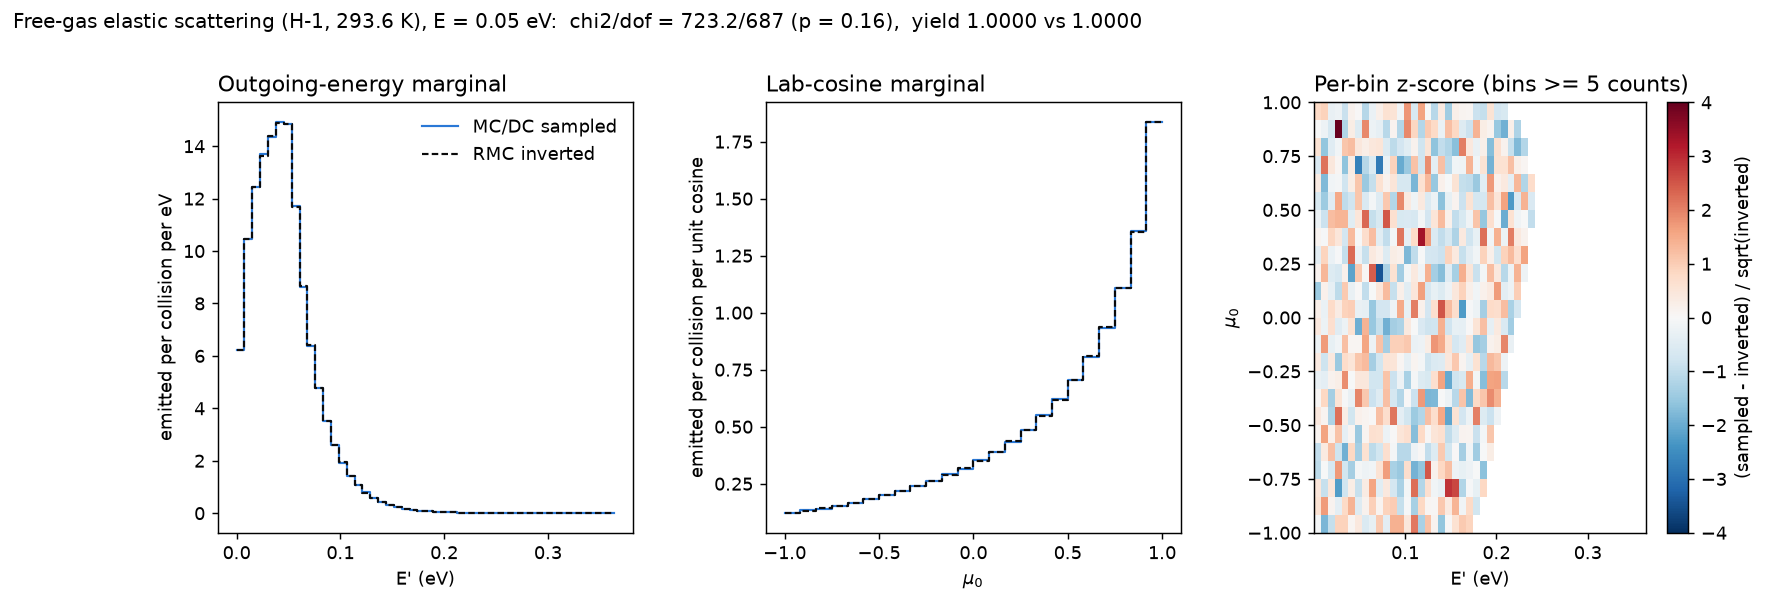
\includegraphics[width=\textwidth]{figures/free_gas_h1/free_gas_h1_E0p05.png}
  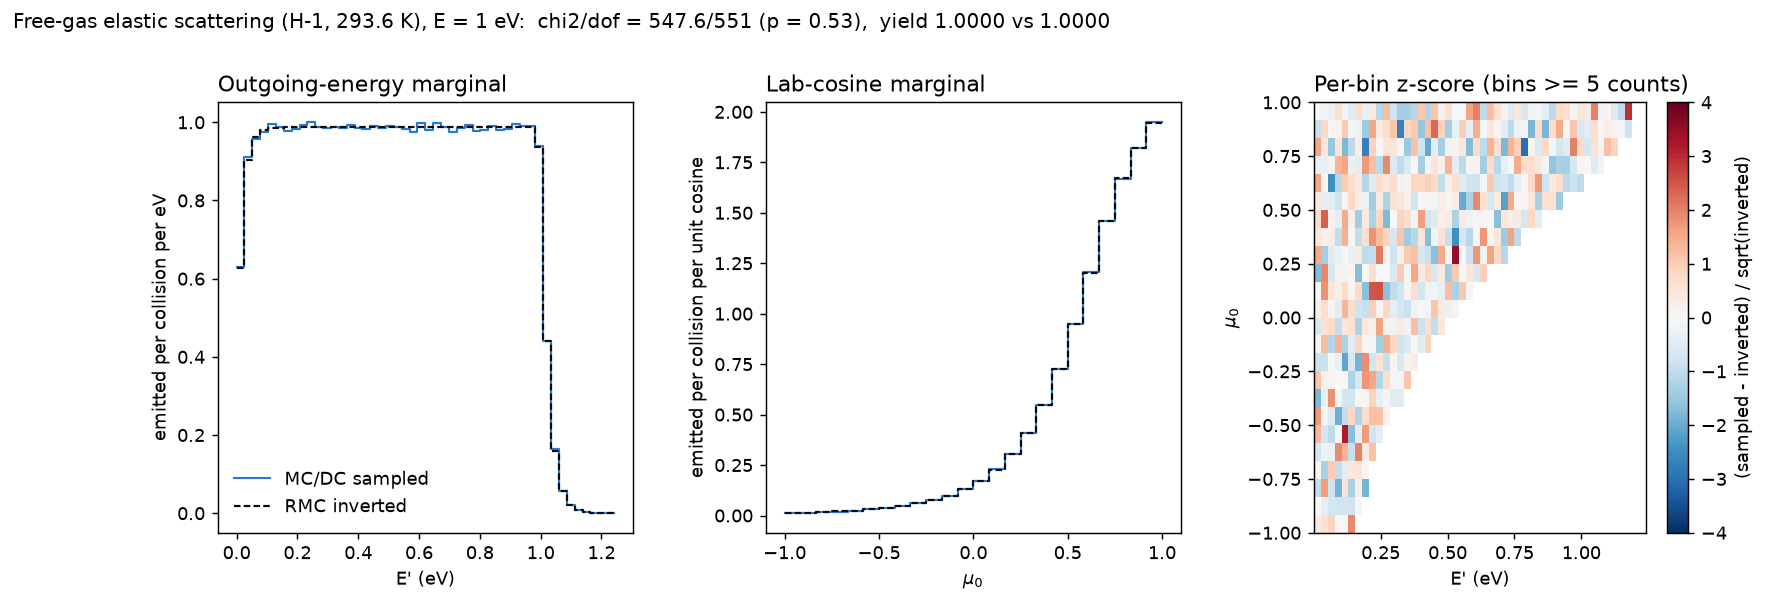
\includegraphics[width=\textwidth]{figures/free_gas_h1/free_gas_h1_E1.png}
  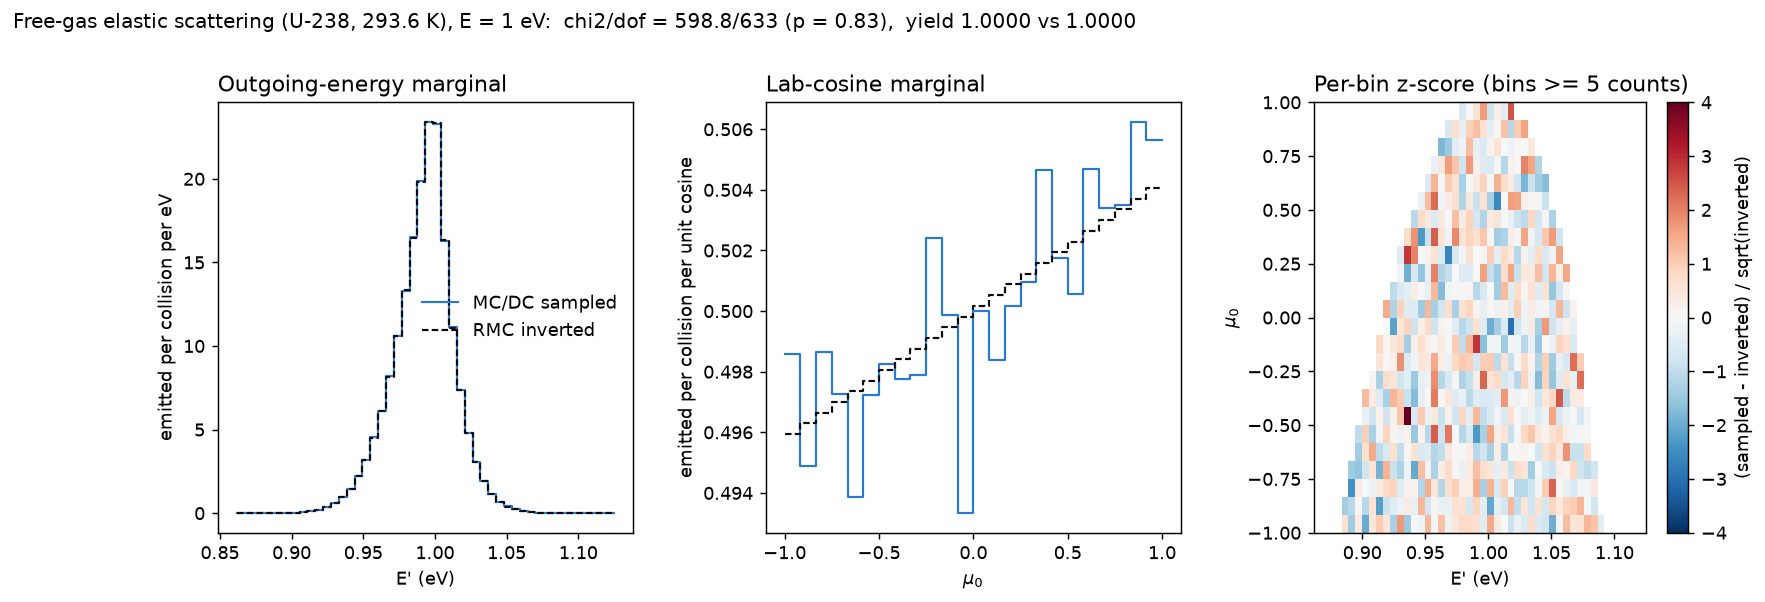
\includegraphics[width=\textwidth]{figures/free_gas_u238/free_gas_u238_E1.png}
  \caption{Free-gas elastic scattering at 293.6\,K: H-1 at 0.05\,eV and 1\,eV
  (broad kernel, strong up-scatter at 0.05\,eV), U-238 at 1\,eV (narrow kernel).}
\end{figure}

\end{document}
